\documentclass{article}
\usepackage{style-assessments}

% define macros (/shortcuts)
% define macros (/shortcuts)
\newcommand{\bu}[1]{\textbf{\ul{#1}}}				% shortcut bold and underline text in one command
\newcommand{\follow}[1]{\sim \text{#1}\,}		% shortcut for ~ 'Named dist ' in normal font with space before parameters would go
\newcommand{\followsp}[2]{\overset{#1}\sim \text{#2}\,}		% (followsp is short for 'follow special') shortcut that can be used for iid or ind ~ 'Named dist ' in normal font with space before parameters would go
\newcommand{\vecn}[2]{#1_1, \ldots, #1_{#2}}	% define vector (without parentheses, so when writing out in like a definition) of the form X_1, ..., X_n, where X and n are variable. NOTE: to call use $\vecn{X}{n}$
\newcommand{\ind}{\perp \!\!\! \perp}			% define independence symbol (it basically makes two orthogonal symbols very close to each other. The number of \! controls the space between each of the orthogonal symbols)
\newcommand{\ho}{H_0}		% shortcut for null hypothesis formatted nicely
\newcommand{\ha}{H_A}		% shortcut for alternative hypothesis formatted nicely



\begin{document}

\begin{center}
{\Huge MATH 321: Test 3 Study Guide}

\end{center}

\bigskip\bigskip

{\large \bu{Lecture 5 -- The Central Limit Theorem}} (5.6 and 5.7)\bigskip

Convergence in distribution
\begin{itemize}
    \item Definition: A sequence of random variables, $Y_1, Y_2, \dots,$ converges in distribution to a random variable $Y$ if $\lim_{n \to \infty} F_{Y_n}(y) = F_Y(y)$ at all points $y$ where $F_Y(y)$ is continuous (notation: $Y_n \overset{d}{\to} Y$).
\end{itemize}\bigskip
        
CLT
\begin{itemize}
    \item[] Central Limit Theorem: Let $X_i \followsp{iid}{$f(x)$}$ with $E(X) = \mu$ and $V(X) = \sigma^2 > 0$. Then the distribution of
    \item[] $\displaystyle W = \frac{\bar{X} - \mu}{\sigma / \sqrt{n}} \follow{Normal}(0,1) \quad \text{as } n \to \infty$
    \item Normal mgf theorem: If $Z \follow{N}(\mu = 0, \sigma^2 = 1)$, and $\mu$ and $\sigma > 0$ are constants, then
    \item[] $X = \sigma Z + \mu \follow{N}(\mu, \sigma^2)$
    \item Results of CLT
    \begin{enumerate}[(a)]
        \item $\displaystyle \frac{\sigma}{\sqrt{n}} W + \mu = \bar{X}$ can be approximated by \\ $\displaystyle \frac{\sigma}{\sqrt{n}} Z + \mu \follow{Normal}(\mu, \frac{\sigma^2}{n})$ for ``large'' $n$.
        \item $n \bar{X} = X_1 + \ldots + X_n = S$ can be approximated by \\ $(\sigma \sqrt{n}) Z + n \mu \follow{Normal}(n \mu, n \sigma^2)$ for ``large'' $n$.
    \end{enumerate}        
\end{itemize}\bigskip

$t$, $Z$, and the CLT
\begin{itemize}
    \item If $\vecn{X}{n}$ are a random sample for a $N(\mu, \sigma^2)$, as $n \to \infty$, $t_{n-1} \overset{d} \to Z$
    \item If $\vecn{X}{n}$ are not normal random variables, when the sample size is large
    \item[] $\displaystyle \frac{\bar{X} - \mu}{S / \sqrt{n}} \followsp{approx}{Normal}(0,1) = Z \quad \text{by CLT}$
\end{itemize}\bigskip

Normal approximation to discrete distributions
\begin{itemize}
    \item Continuity correction: If $X \follow{Discrete}$ with corresponding $S \follow{Normal}$ by the CLT, then for integers $a \le b$:
    \item[] $P(X = a) = P(a - 0.5 \le S \le a + 0.5)$ \hspace{20pt} and \hspace{20pt} $P(a \le X \le b) = P(a - 0.5 \le S \le b + 0.5)$
    \item Normal approximation to binomial
    \begin{itemize}
        \item Result: If $X \follow{Binomial}(n,p) \Longrightarrow X \approx S \follow{Normal}(\mu = np, \sigma^2 = npq)$
        \item Conditions: $np \ge 5$ and $nq = n(1 - p) \ge 5$
    \end{itemize}
    \item Normal approximation to Poisson
    \begin{itemize}
        \item Result: If $X \follow{Poisson}(\lambda) \Longrightarrow X \approx S \follow{Normal}(\mu = \lambda, \sigma^2 = \lambda)$
        \item Condition: $\lambda \ge 10$
    \end{itemize}
\end{itemize}

\newpage

Central interval probabilities
\begin{itemize}
    \item Empirical rule: If $X \followsp{approx}{Normal}$, then
    \begin{enumerate}
        \item Approximately 68\% of data is within $\mu \pm \sigma$
        \item Approximately 95\% of data is within $\mu \pm 2\sigma$
        \item Approximately 99.7\% of data is within $\mu \pm 3\sigma$
    \end{enumerate}
\end{itemize}\bigskip

\vspace{50pt}

{\large \bu{Lecture 6 -- Confidence Intervals}} (7.1 - 7.4)\bigskip

Interval estimators / confidence intervals
\begin{itemize}
    \item Definition: An interval estimator or confidence interval for how to calculate endpoints of an interval from sample data: $[L(\mathbf{X}), U(\mathbf{X})]$
    \item[] Once $\mathbf{X} = \mathbf{x}$ is observed, the inference $L(\mathbf{x}) \le \theta \le U(\mathbf{x})$ is made.
    \item Goals of CIs: (1) Capture the target parameter $\theta$ (2) Be relatively narrow
    \item Confidence coefficients definition:
    \item[] Probability that a CI captures $\theta$ $\rightarrow$ $P\big(L(\mathbf{X}) \le \theta \le U(\mathbf{X})\big) = 1 - \alpha$ for significance level $\alpha$
    \item $100 (1 - \alpha)\%$ CI for $\theta$ = $[L(\mathbf{X}), U(\mathbf{X})]$   
\end{itemize}\bigskip

Constructing confidence intervals
\begin{itemize}    
    \item Setup: $\hat{\theta}$ = unbiased point estimator for parameter $\theta$; \\ $\sigma_{\hat{\theta}}$ = standard deviation of the sampling distribution of $\hat{\theta}$ (i.e. standard error of $\hat{\theta}$)
    \item[] If $\hat{\theta} \follow{Normal}(\theta, \sigma_{\hat{\theta}})$ (or approximately normal) $\Longrightarrow$ $Z = \frac{\hat{\theta} - \theta}{\sigma_{\hat{\theta}}} \follow{Normal}(0,1)$
    \item To find interval for $\theta$ with confidence coefficient equal to $1 - \alpha$, need critical values $-z_{\alpha / 2}$ and $z_{\alpha / 2}$ such that $P(-z_{\alpha / 2} \le Z \le z_{\alpha / 2}) = 1 - \alpha$. Then 
    
        \begin{align*}
         1 - \alpha &= P(-z_{\alpha / 2} \le Z \le z_{\alpha / 2}) \\
             &= P(-z_{\alpha / 2} \le \frac{\hat{\theta} - \theta}{\sigma_{\hat{\theta}}} \le z_{\alpha / 2}) \\
             & = P(\hat{\theta} - z_{\alpha / 2} \, \sigma_{\hat{\theta}} \le \theta \le \hat{\theta} + z_{\alpha / 2} \, \sigma_{\hat{\theta}}) \\
             &\Longrightarrow 100 (1 - \alpha)\% \text{ CI } = [\hat{\theta} - z_{\alpha / 2} \, \sigma_{\hat{\theta}}, \hat{\theta} + z_{\alpha / 2} \, \sigma_{\hat{\theta}}] \\
             &= \hat{\theta} \pm z_{\alpha / 2} \, \sigma_{\hat{\theta}} \\
    \end{align*}

    \begin{figure}[H]
    \begin{minipage}{0.45\textwidth}
        \center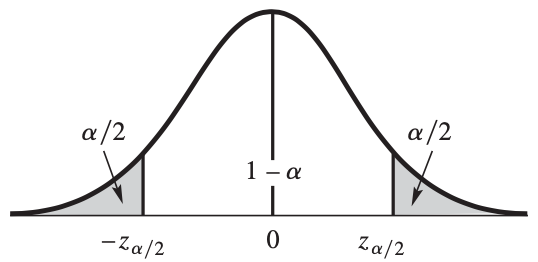
\includegraphics[scale=0.5]{images/z-critical-values.png}
    \end{minipage}
    \begin{minipage}{0.4\textwidth}
        \center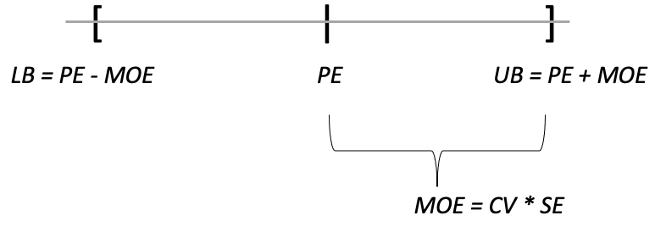
\includegraphics[scale=0.5]{images/ci-general.png}
    \end{minipage}
    \end{figure}

    \item Summary of CIs
    \begin{itemize}
        \item Point Estimate (PE) is the best guess; at the center of the interval.
        \item Margin of Error (MOE) = Critical Value (CV) $\times$ Standard Error (SE).
        \item[] SE (standard deviation of the statistic) measures sampling error.
        \item[] \% Confident is determined by confidence level set and incorporated via the critical value (CV).
    \end{itemize}
    \item All else equal, here is how the researcher can affect the precision of intervals:
    \begin{itemize}
        \item Larger sample size $n$ $\rightarrow$ smaller interval (smaller SE)
        \item More confident $\rightarrow$ larger interval (larger CV)
        \begin{figure}[H]
            \center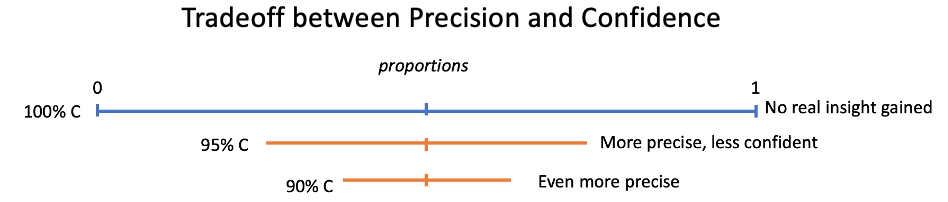
\includegraphics[scale=0.5]{images/confidence-vs-precision.png}
        \end{figure}
    \end{itemize}
    \item Interpretation general structure:
    \item[] I am \ul{\% confident} that the true/population \ul{parameter + context} is between \\ \ul{lower bound} and \ul{upper bound}.
\end{itemize}\bigskip

Types of intervals
\begin{itemize}
    \item Variables that affect the form of intervals:
    \begin{itemize}
        \item Independent or dependent samples
        \item Sample sizes $n_1$ and $n_2$ (large or small)
        \item Population distributions $X_1$ and $X_2$ (normal or not normal)
        \item Population variances $\sigma^2_1$ and $\sigma^2_2$ (known or unknown and ratio of variances)
    \end{itemize}
    \item Large sample confidence intervals
    \item[] If $n$ is large $\Longrightarrow$ $\hat{\theta} \followsp{approx}{Normal}(\theta, \sigma_{\hat{\theta}}) \Longrightarrow 100 (1 - \alpha)\% \text{ CI } = \hat{\theta} \pm z_{\alpha / 2} \, \sigma_{\hat{\theta}}$
    \item[] Conditions: for means $n_i \ge 30$; for proportions $n_i p_i \ge 5$ and $n_i (1 - p_i) \ge 5$ \bigskip\\
    \begin{tabular}{llll}
    $\theta$ & $\hat{\theta}$ & $\sigma_{\hat{\theta}}$ & \\
    \hline\\
    $\mu$ & $\bar{X}$ & $\displaystyle \frac{\sigma}{\sqrt{n}}$ & Estimate $\sigma^2$ with $s^2$ if unknown \\\\
    $\mu_1 - \mu_2$ & $\bar{X}_1 - \bar{X}_2$ & $\displaystyle \sqrt{\frac{\sigma^2_1}{n_1} + \frac{\sigma^2_2}{n_2}}$ & Estimate $\sigma^2_i$ with $s^2_i$ if unknown \\\\
    $p$ & $\hat{p}$ & $\displaystyle \sqrt{\frac{p (1 - p)}{n}}$ & Estimate $p$ with $\hat{p}$ \\\\
    $p_1 - p_2$ & $\hat{p}_1 - \hat{p}_2$ & $\displaystyle \sqrt{\frac{p_1 (1 - p_1)}{n_1} + \frac{p_2 (1 - p_2)}{n_2}}$ & Estimate $p_i$ with $\hat{p}_i$ \\\\
    \end{tabular}
    \item[] If starting from $X_i \follow{Normal}$ and known variances, then intervals are exact; if not then $X_i \approx \text{Normal}$ by CLT and confidence coefficients are approximate.\newpage
    \item Small sample confidence intervals for means ($n_i < 30$)
    \item[] If $n$ is small $\Longrightarrow$ $100 (1 - \alpha)\% \text{ CI } = \hat{\theta} \pm t_{\alpha / 2} \, \sigma_{\hat{\theta}}$ \hspace{100pt} $t$ crit values > $z$ crit values
    \item[] Conditions: for one sample $X \follow{Normal}$ with unknown $\sigma^2$; for two samples $X_1 \ind X_2$ and \\ $X_1, X_2 \follow{Normal}$ with unknown common variance $\sigma^2$
    \begin{figure}[H]
        \center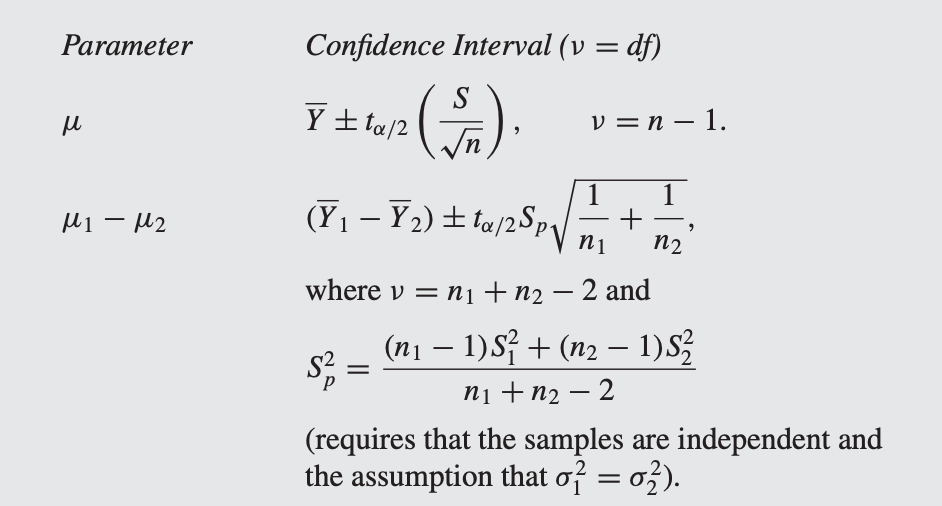
\includegraphics[scale=0.5]{images/small-n-ci.png}
    \end{figure}
    \item[] If not starting from $X_i \follow{Normal}$ then confidence coefficients are approximate and work well as long as not badly skewed with outliers.
    \item Dependent samples CI for $\mu_1 - \mu_2$
    \item[] Simplifies to a one sample CI for the differences $\mu_1 - \mu_ 2 = \mu_D$ shown above if $n$ is small\bigskip
    \item One-sided CI
    \item[] \ul{Lower bound (at least)} \hspace{200pt} \ul{Upper bound (at most)}
    \item[] $P(\hat{\theta} - z_\alpha \, \sigma_{\hat{\theta}}) = 1 - \alpha$  \hspace{150pt} $P(\hat{\theta} + z_\alpha \, \sigma_{\hat{\theta}}) = 1 - \alpha$
    \item[] $\Longrightarrow [\hat{\theta} - z_\alpha \, \sigma_{\hat{\theta}}, \infty)$ \hspace{170pt} $\Longrightarrow (-\infty, \hat{\theta} + z_\alpha \, \sigma_{\hat{\theta}}]$
\end{itemize}\bigskip

Margin of error (MOE) revisited
\begin{itemize}
    \item $MOE = \frac{UB - LB}{2} = \frac{Width}{2} \hspace{20pt} \rightarrow \hspace{20pt} Width = 2 \times MOE$
    \item The \textbf{error in estimation} $\boldsymbol{\epsilon}$ is the distance between an estimator and its target parameter:
    \item[] $[\hat{\theta} - \epsilon, \hat{\theta} + \epsilon] \Longrightarrow \lvert \hat{\theta} - \theta \rvert = \epsilon$
\end{itemize}\bigskip

Finding minimum sample size
\begin{itemize}
    \item We want the $100 (1 - \alpha)\%$ confidence interval for $\theta$, $\hat{\theta} \pm z_{\alpha / 2} \sigma_{\hat{\theta}}$, to be no longer than that given by $\hat{\theta} \pm \epsilon$, then for
    \begin{itemize}
        \item One mean $\mu$ with $V(X) = \sigma^2$ known and $X \follow {Normal}$ or assume going to have ``large'' $n$:
        \item[] $\displaystyle n \ge \frac{z_{\alpha / 2}^2 \sigma^2}{\epsilon^2}$
        \item[] If $\sigma^2$ is unknown, use best approximation available.
        \item One proportion $p$: $\displaystyle n \ge \frac{z_{\alpha / 2}^2 \, p^* (1 - p^*)}{\epsilon^2}$
        \item[] If there is prior knowledge, use $p^* = \hat{p}$, else set $p^* = 0.5$
    \end{itemize}
\end{itemize}

\newpage

{\large \bu{Lecture 7 -- Hypothesis Tests}} (8.1 - 8.3)\bigskip

Hypothesis test
\begin{itemize}
    \item Definition: A hypothesis test is a rule that specifies
    \item[] For which sample value the decision is made to reject $\ho$ in favor of $\ha$.
    \item[] For which sample value the decision is made to ``not reject'' $\ha$ in favor of $\ha$.
    \item Elements of a hypothesis test
    \begin{enumerate}
        \item Null hypothesis $\ho$ and Alternative hypothesis $\ha$
        \item[] Definitions:
        \begin{itemize}
            \item Hypotheses are statements about population parameters
            \item The Null hypothesis $\ho$ is an assumption about $\theta$ that is assumed to be true
            \item The Alternative hypothesis $\ha$ is the complement of $\ho$
        \end{itemize}
        \item Test statistic (TS) and Rejection Region $RR$
        \item[] TS: Function of the sample $W(\vecn{X}{n})$, think of this as the point estimator $\hat{\theta}$
        \item[] RR: Subset of the sample space (range of sample) for which $\ho$ will be rejected
        \item Conclusion / interpretation
        \item[] General structure: Because our test statistic \ul{(COMPARISON of TS and RR)} \ul{(IS / IS NOT)} in the rejection region we \ul{(REJECT or FAIL TO REJECT)} the null hypothesis. \\ At the \ul{(ALPHA)} significance level, there \ul{(IS or IS NOT)} sufficient evidence to conclude \ul{(THE ALTERNATIVE HYPOTHESIS)}.
    \end{enumerate}
\end{itemize}\bigskip

Large sample tests
\begin{itemize}
    \item If $n$ is large, then $\hat{\theta} \follow{Normal}(\theta, \sigma_{\hat{\theta}})$ (or approximately normal) $\Longrightarrow$ $Z = \frac{\hat{\theta} - \theta}{\sigma_{\hat{\theta}}} \follow{Normal}(0,1)$
    \item Using the same parameters $\theta$, point estimates $\hat{\theta}$, and standard errors $\sigma_{\hat{\theta}}$ as shown in confidence intervals, all of the large sample $\alpha$-level tests can be summarized with
    \begin{figure}[H]
    \begin{minipage}{0.45\textwidth}
        \center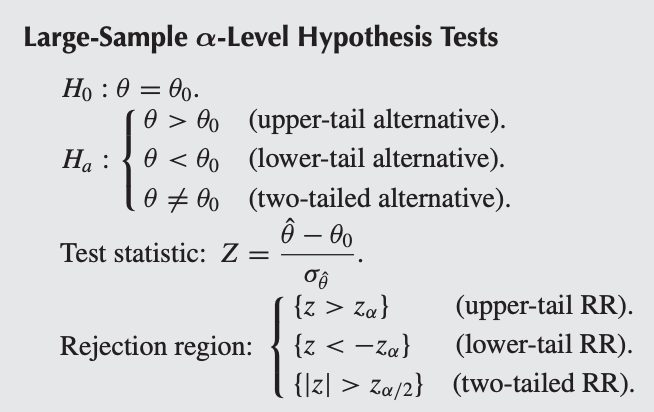
\includegraphics[scale=0.5]{images/large-sample-tests-summary.png}
    \end{minipage}
    \begin{minipage}{0.4\textwidth}
        \center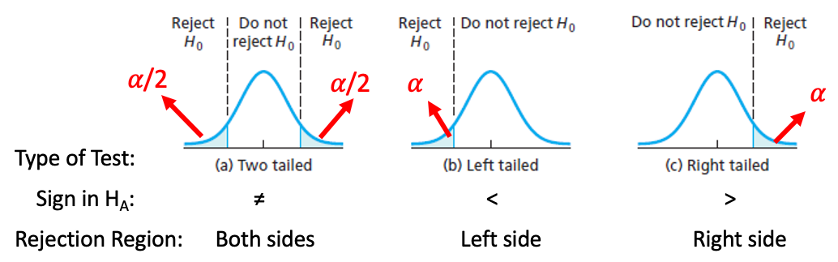
\includegraphics[scale=0.4]{images/rr.png}
    \end{minipage}
    \end{figure}
    \item For proportions
    \begin{itemize}
        \item One sample: In the standard error, use $p_0$ $\Longrightarrow \displaystyle \sigma_{\hat{p}} = \sqrt{\frac{p_0 (1 - p_0)}{n}}$.
        \item Two sample: In the standard error, use $p_1 = p_2 = p$ and estimate with \\$\displaystyle \hat{p} = \frac{x_1 + x_2}{n_1 + n_2} \Longrightarrow \sigma_{\hat{p}_1 - \hat{p}_2} = \sqrt{\hat{p} (1 - \hat{p}) [1 / n_1 + 1 / n_2]}$.
    \end{itemize}\newpage
    \item In any particular test, only one of the listed alternatives $\ha$ is appropriate, which will be based on the research question. Then use the corresponding rejection region.
\end{itemize}\bigskip

Small sample tests for means
\begin{itemize}
    \item If $n$ is small, then need to switch to $t$-tests. For these we start with $X \follow{Normal}$
    \item Summary of the small-sample $\alpha$-level tests for $\mu$
    \begin{figure}[H]
        \center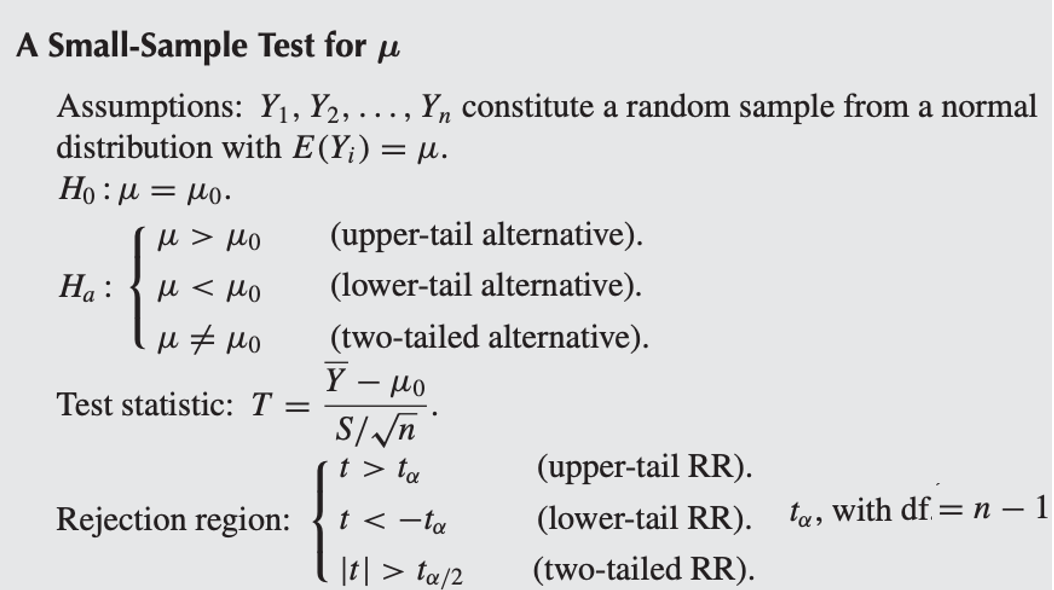
\includegraphics[scale=0.5]{images/small-sample-tests-summary-one-mean.png}
    \end{figure}
    \item If we are testing two independent means $\mu_1 - \mu_2$ and assume both Normal distributions with common unknown variance $\sigma^2$, then we use the pooled variance $S^2_p$ as the estimator for $\sigma^2$ in the standard error $\sigma_{\bar{X}_1 - \bar{X}_2}$. Then
    \begin{figure}[H]
        \center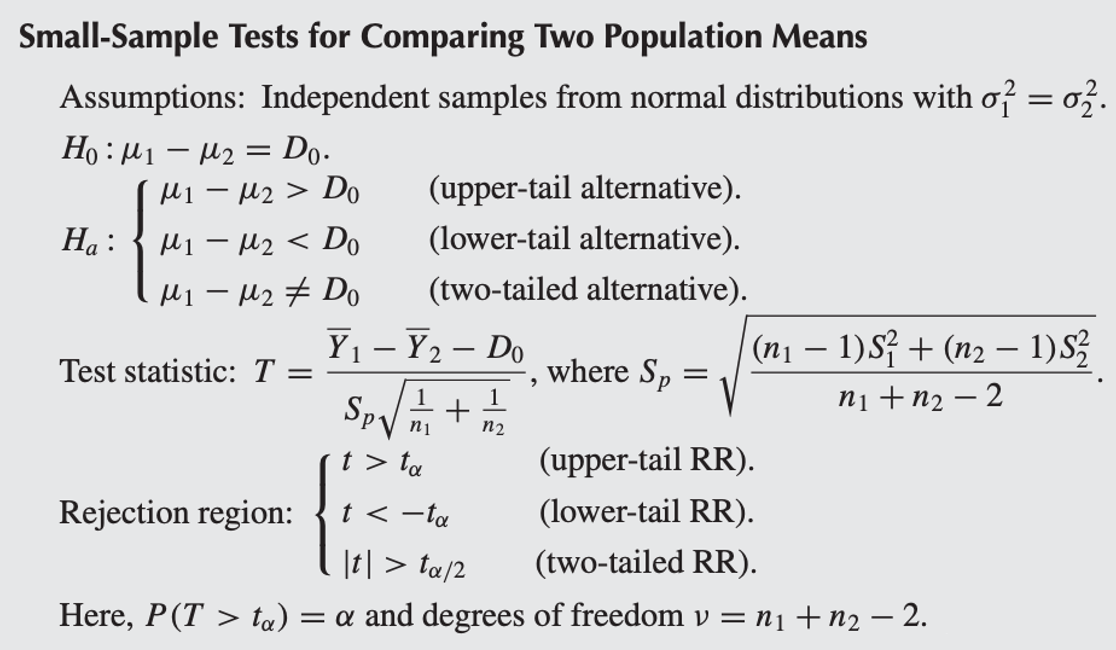
\includegraphics[scale=0.5]{images/small-sample-tests-summary-two-means.png}
    \end{figure}
    \item If we are testing dependent means $\mu_1 - \mu_2$, then have paired $t$-test    \item[] $\mu_1 - \mu_2 = \mu_D \hspace{20pt} \rightarrow \hspace{20pt} \frac{\bar{D} - \mu_D}{S_D / \sqrt{n}} = T \follow{t}_{n-1}$, \hspace{20pt} one sample test on differences
    \item[] If not starting from $X_i \follow{Normal}$ then $t$-tests are approximately $\alpha$-level and work well as long as not badly skewed with outliers.
\end{itemize}\newpage

p-values
\begin{itemize}
    \item Definition: A p-value is the probability that under the null hypothesis the test statistic will be at least as ``extreme'' as the observed value.
    \item Two ways to make conclusion for hypothesis tests:
    \item[] Traditional method: $TS \overset{?}\in RR$
    \item[] p-value method: Reject $\ho$ if p-value $\le \alpha$ \hspace{10pt} and \hspace{10pt} Fail to reject $\ho$ if p-value $> \alpha$
\end{itemize}\bigskip

Relationship between confidence intervals and hypothesis tests
\begin{itemize}
    \item Confidence interval = Acceptance region = Complement of RR
    \item Decisions based on CI: For $\ho: \theta = \theta_0$ and
    \item[] Two-tailed $\ha: \theta \ne \theta_0$: ``Accept'' $\ho$ if $\theta_0$ falls within the $100 (1 - \alpha)$\% CI and reject if outside.
    \item[] Right-tailed $\ha: \theta > \theta_0$: Reject if outside lower bound CI
    \item[] Right-tailed $\ha: \theta < \theta_0$: Reject if outside upper bound CI
\end{itemize}\bigskip

Type I and Type II errors
\begin{itemize}
    \item Type I: Incorrectly rejecting $\ho$
    \item[] $\alpha = P(\text{Type I error}) = P(\text{Reject when $\ho$ is true}) = P(TS \in RR \mid \ho)$
    \item Type II: Incorrectly failing to reject $\ho$
    \item[] $\beta = P(\text{Type II error}) = P(\text{Fail to reject when $\ho$ is false}) = P(TS \notin RR \mid \ha)$
    \begin{figure}[H]
        \center Example for one mean
        \center\includegraphics[scale=0.5]{{"images/type1-type2"}.png}
    \end{figure}
    \item Power: Correctly rejecting $\ho$
    \item[] $\text{Power} = 1 - \beta = P(\text{Reject $\ho$ when $\ho$ is false}) = P(TS \in RR \mid \ha)$
\end{itemize}



% same distribution table as last test -> so skipping here

\end{document}




